% Author: Izaak Neutelings (Februari, 2020)
% page 8 https://archive.org/details/StaticAndDynamicElectricity
% https://tex.stackexchange.com/questions/56353/extract-x-y-coordinate-of-an-arbitrary-point-on-curve-in-tikz
% https://tex.stackexchange.com/questions/412899/tikz-calculate-and-store-the-euclidian-distance-between-two-coordinates

\documentclass[border=3pt,tikz]{standalone}
\usepackage{amsmath} % for \dfrac
\usepackage{physics}
\usepackage{tikz,pgfplots}
\usetikzlibrary{angles,quotes} % for pic (angle labels)
\usetikzlibrary{decorations.markings}
\tikzset{>=latex} % for LaTeX arrow head

\usepackage{xcolor}
\colorlet{Ecol}{orange!90!black}
\colorlet{veccol}{green!45!black}
\tikzstyle{EField}=[thick,Ecol]
\def\xmax{5.0}
\def\ymax{3.3}
\def\tick#1#2{\draw[thick] (#1) ++ (#2:0.03*\ymax) --++ (#2-180:0.06*\ymax)}


\begin{document}


% ELECTRIC FIELD of a ROD
\begin{tikzpicture}
  
  \def\kQ{2.0}
  \coordinate (O) at (0,0);
  \coordinate (X) at (\xmax,0);
  \coordinate (Y) at (0,\ymax);
  
  % AXIS
  \draw[<->,thick]
    (X) node[below] {$y$} -- (O) -- (Y) node[left] {$E$};
  
  % PLOT
  \draw[EField,samples=100,smooth,variable=\x,domain={1.1*\kQ/\ymax}:0.96*\xmax]
    plot(\x,\kQ/\x);
  \node[above right] at (1.3,1.6) {$E \sim \dfrac{1}{y}$};
  
\end{tikzpicture}


% ELECTRIC FIELD of a ROD
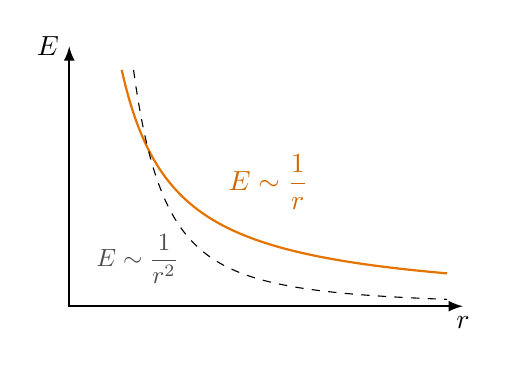
\begin{tikzpicture}
  
  \def\kQ{2.0}
  \coordinate (O) at (0,0);
  \coordinate (X) at (\xmax,0);
  \coordinate (Y) at (0,\ymax);
  
  % AXIS
  \draw[<->,thick]
    (X) node[below] {$r$} -- (O) -- (Y) node[left] {$E$};
  
  % PLOT
  \draw[EField,samples=100,smooth,variable=\x,domain={1.1*\kQ/\ymax}:0.96*\xmax]
    plot(\x,\kQ/\x);
  \draw[black!70,thin,dashed,black,samples=100,smooth,variable=\x,domain={sqrt(1.1*\kQ/\ymax)}:0.96*\xmax]
    plot(\x,\kQ/\x^2);
  \node[black!70,left,scale=0.9] at (1.5,0.6) {$E \sim \dfrac{1}{r^2}$}; %(0.9,2.9)
  \node[Ecol!90!black,above right] at (1.9,1.1) {$E \sim \dfrac{1}{r}$};
  
\end{tikzpicture}


% ELECTRIC FIELD of a PLANE
\begin{tikzpicture}
  
  \def\kQ{2.3}
  \coordinate (O) at (0,0);
  \coordinate (X) at (\xmax,0);
  \coordinate (Y) at (0,\ymax);
  
  % AXIS
  \draw[<->,thick]
    (X) node[below] {$x$} -- (O) -- (Y) node[left] {$E$};
  \tick{0,\kQ}{ 0} node[below=-1,left] {$\dfrac{\sigma}{2\epsilon_0}$};
  
  % PLOT
  \draw[EField,samples=100,smooth,variable=\x,domain=0:0.96*\xmax]
    plot(\x,\kQ);
  \draw[black!60,thin,dashed,black,samples=100,smooth,variable=\x,domain={sqrt(1.1*\kQ/\ymax)}:0.96*\xmax]
    plot(\x,\kQ/\x^2);
  \node[black!60,left,scale=0.9] at (3.2,1.2) {$E \sim \dfrac{1}{x^2}$};
  
\end{tikzpicture}


% ELECTRIC FIELD of a CHARGED, SOLID SPHERE
% or ELECTRIC FIELD of a CONDUCTING SPHERE with excess charge
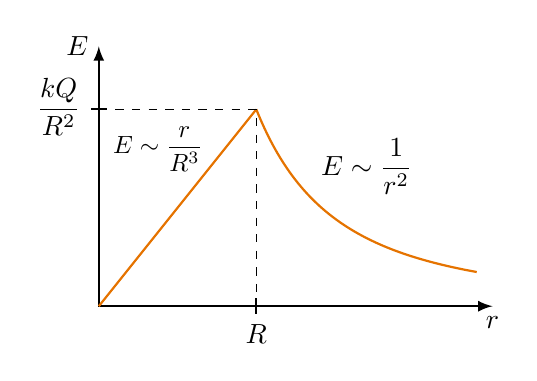
\begin{tikzpicture}
  
  \def\kQ{10}
  \def\R{2.0}
  \coordinate (O) at (0,0);
  \coordinate (X) at (\xmax,0);
  \coordinate (Y) at (0,\ymax);
  \coordinate (P) at (\R,\kQ/\R^2);
  \coordinate (Px) at (\R,0);
  \coordinate (Py) at (0,\kQ/\R^2);
  
  % AXIS
  \draw[<->,thick]
    (X) node[below] {$r$} -- (O) -- (Y) node[left] {$E$};
  \tick{Py}{ 0} node[below=-1,left] {$\dfrac{kQ}{R^2}$};
  \tick{Px}{90} node[below] {$R$};
  
  % PLOT
  \draw[EField,samples=100,smooth,variable=\x,domain=0:\R]
    plot(\x,\kQ*\x/\R^3);
  \draw[EField,samples=100,smooth,variable=\x,domain=\R:0.96*\xmax]
    plot(\x,\kQ/\x^2);
  \node[scale=0.9] at (0.75,2.0) {$E \sim \dfrac{r}{R^3}$};
  \node[above right] at (2.7,1.3) {$E \sim \dfrac{1}{r^2}$};
  \draw[dashed]
    (Py) -- (P) -- (Px);
  
\end{tikzpicture}


% ELECTRIC FIELD of a CHARGED SPHERE
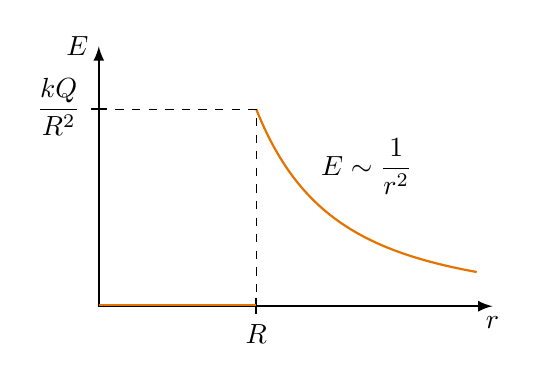
\begin{tikzpicture}
  
  \def\kQ{10}
  \def\R{2.0}
  \coordinate (O) at (0,0);
  \coordinate (X) at (\xmax,0);
  \coordinate (Y) at (0,\ymax);
  \coordinate (P) at (\R,\kQ/\R^2);
  \coordinate (Px) at (\R,0);
  \coordinate (Py) at (0,\kQ/\R^2);
  
  % AXIS
  \draw[<->,thick]
    (X) node[below] {$r$} -- (O) -- (Y) node[left] {$E$};
  \tick{Py}{ 0} node[below=-1,left] {$\dfrac{kQ}{R^2}$};
  \tick{Px}{90} node[below] {$R$};
  
  % PLOT
  \draw[EField,samples=100,smooth,variable=\x,domain=\R:0.96*\xmax]
    plot(\x,\kQ/\x^2);
  \draw[EField]
    (0,0.004*\ymax) --++ (Px);
  \node[above right] at (2.7,1.3) {$E \sim \dfrac{1}{r^2}$};
  \draw[dashed]
    (Py) -- (P) -- (Px);
  
\end{tikzpicture}


% ELECTRIC FIELD of a CONDUCTING SLAB
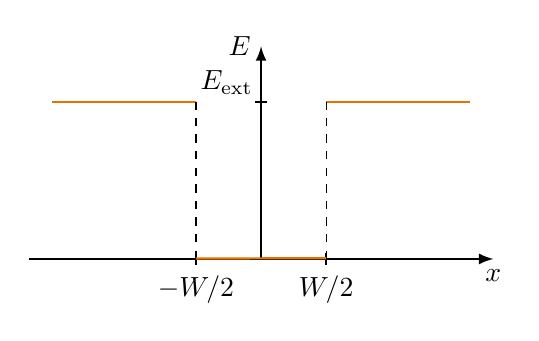
\begin{tikzpicture}
  
  \def\xmax{5.9}
  \def\ymax{2.7}
  \def\E{0.74*\ymax}
  \def\W{0.28*\xmax}
  
  \coordinate (O) at (0,0);
  \coordinate (XL) at (-\xmax/2,0);
  \coordinate (XR) at (\xmax/2,0);
  \coordinate (Y) at (0,\ymax);
  
  % AXIS
  \draw[->,thick]
    (XL) -- (XR) node[below] {$x$};
  \draw[->,thick]
    (O) -- (Y) node[left] {$E$};
  \tick{-\W/2,0}{90} node[below] {$-W/2$};
  \tick{\W/2,0}{90} node[below] {$W/2$};
  \tick{0,\E}{0} node[above=2,above left=-3] {$E_\text{ext}$};
  
  % PLOT
  \draw[EField]
    (-0.45*\xmax,\E) -- (-\W/2,\E);
  \draw[EField]
    (\W/2,\E) -- (0.45*\xmax,\E);
  \draw[dashed]
    (-\W/2,0) -- (-\W/2,\E);
  \draw[dashed]
    ( \W/2,0) -- ( \W/2,\E);
  \draw[EField]
    (-\W/2,0.005) -- (\W/2,0.01);
    
\end{tikzpicture}



% ELECTRIC FIELD of a CONDUCTING SPHERE with a cavity
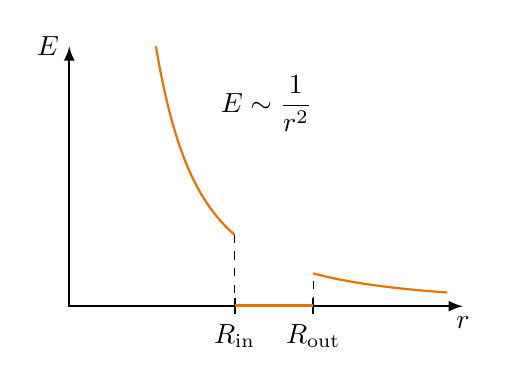
\begin{tikzpicture}
  
  \def\kQ{4}
  \def\Rin{2.1}
  \def\Rout{3.1}
  \coordinate (O) at (0,0);
  \coordinate (X) at (\xmax,0);
  \coordinate (Y) at (0,\ymax);
  
  % AXIS
  \draw[<->,thick]
    (X) node[below] {$r$} -- (O) -- (Y) node[left] {$E$};
  \tick{\Rin,0}{90} node[below] {$R_\text{in}$};
  \tick{\Rout,0}{90} node[below] {$R_\text{out}$};
  
  % PLOT
  \draw[EField,samples=100,smooth,variable=\x,domain={sqrt(1.0*\kQ/\ymax)}:\Rin]
    plot (\x,\kQ/\x^2);
  \draw[dashed]
    (\Rin,\kQ/\Rin^2) -- (\Rin,0.01);
  \draw[EField]
    (\Rin,0.01) -- (\Rout,0.01);
  \draw[dashed]
    (\Rout,0.01) -- (\Rout,\kQ/\Rout^2);
  \draw[EField,samples=100,smooth,variable=\x,domain=\Rout:0.96*\xmax]
    plot (\x,\kQ/\x^2);
  \node[above right] at (1.8,2.1) {$E \sim \dfrac{1}{r^2}$};
  
\end{tikzpicture}



\end{document}
